% ============================================================================
% SECCIÓN 5.8: BASE METODOLÓGICA DEL SISTEMA DE INFERENCIA DIFUSA
% ============================================================================
% VERSIÓN CORREGIDA: FUNCIONES TRIANGULARES (NO TRAPEZOIDALES)
% Autor: Atlas (Científico de Datos Biomatemático Jr.)
% Fecha: 15 de Noviembre de 2025
% Reemplaza: Líneas 450-481 de 05_materiales_metodos.tex
% ============================================================================

\section{Base Metodológica del Sistema de Inferencia Difusa}
\label{sec:base_metodologica_sistema_difuso}

Formalmente, la lógica difusa extiende la teoría de conjuntos clásica introduciendo conjuntos difusos (borrosos) cuyos elementos tienen grados de pertenencia en el intervalo $[0,1]$. Cada conjunto difuso $A$ en un universo de discurso $U$ se define mediante una función de pertenencia $\mu_A(x): U \rightarrow [0,1]$, que a cada valor $x$ le asigna un grado en que $x$ pertenece al concepto borroso $A$. Un grado $\mu_A(x) = 1$ indica pertenencia plena, $\mu_A(x) = 0$ indica no pertenencia, y valores intermedios reflejan pertenencia parcial.

Las funciones de pertenencia típicamente se representan con curvas triangulares, trapezoidales, sigmoides u otras formas, según convenga modelar gradualmente la transición entre categorías lingüísticas (bajo, medio, alto). En el presente estudio, se adoptaron \textbf{funciones de membresía triangulares} debido a su parsimonia matemática, interpretabilidad clínica directa, y robustez ante tamaños muestrales pequeños. La \Cref{fig:funciones_membresia} muestra las funciones triangulares definidas para cada variable de entrada del sistema, con tres categorías lingüísticas por variable cuyos parámetros fueron determinados mediante percentiles empíricos de la cohorte (data-driven) complementados con criterios fisiológicos para garantizar relevancia clínica.

\begin{figure}[htbp]
    \centering
    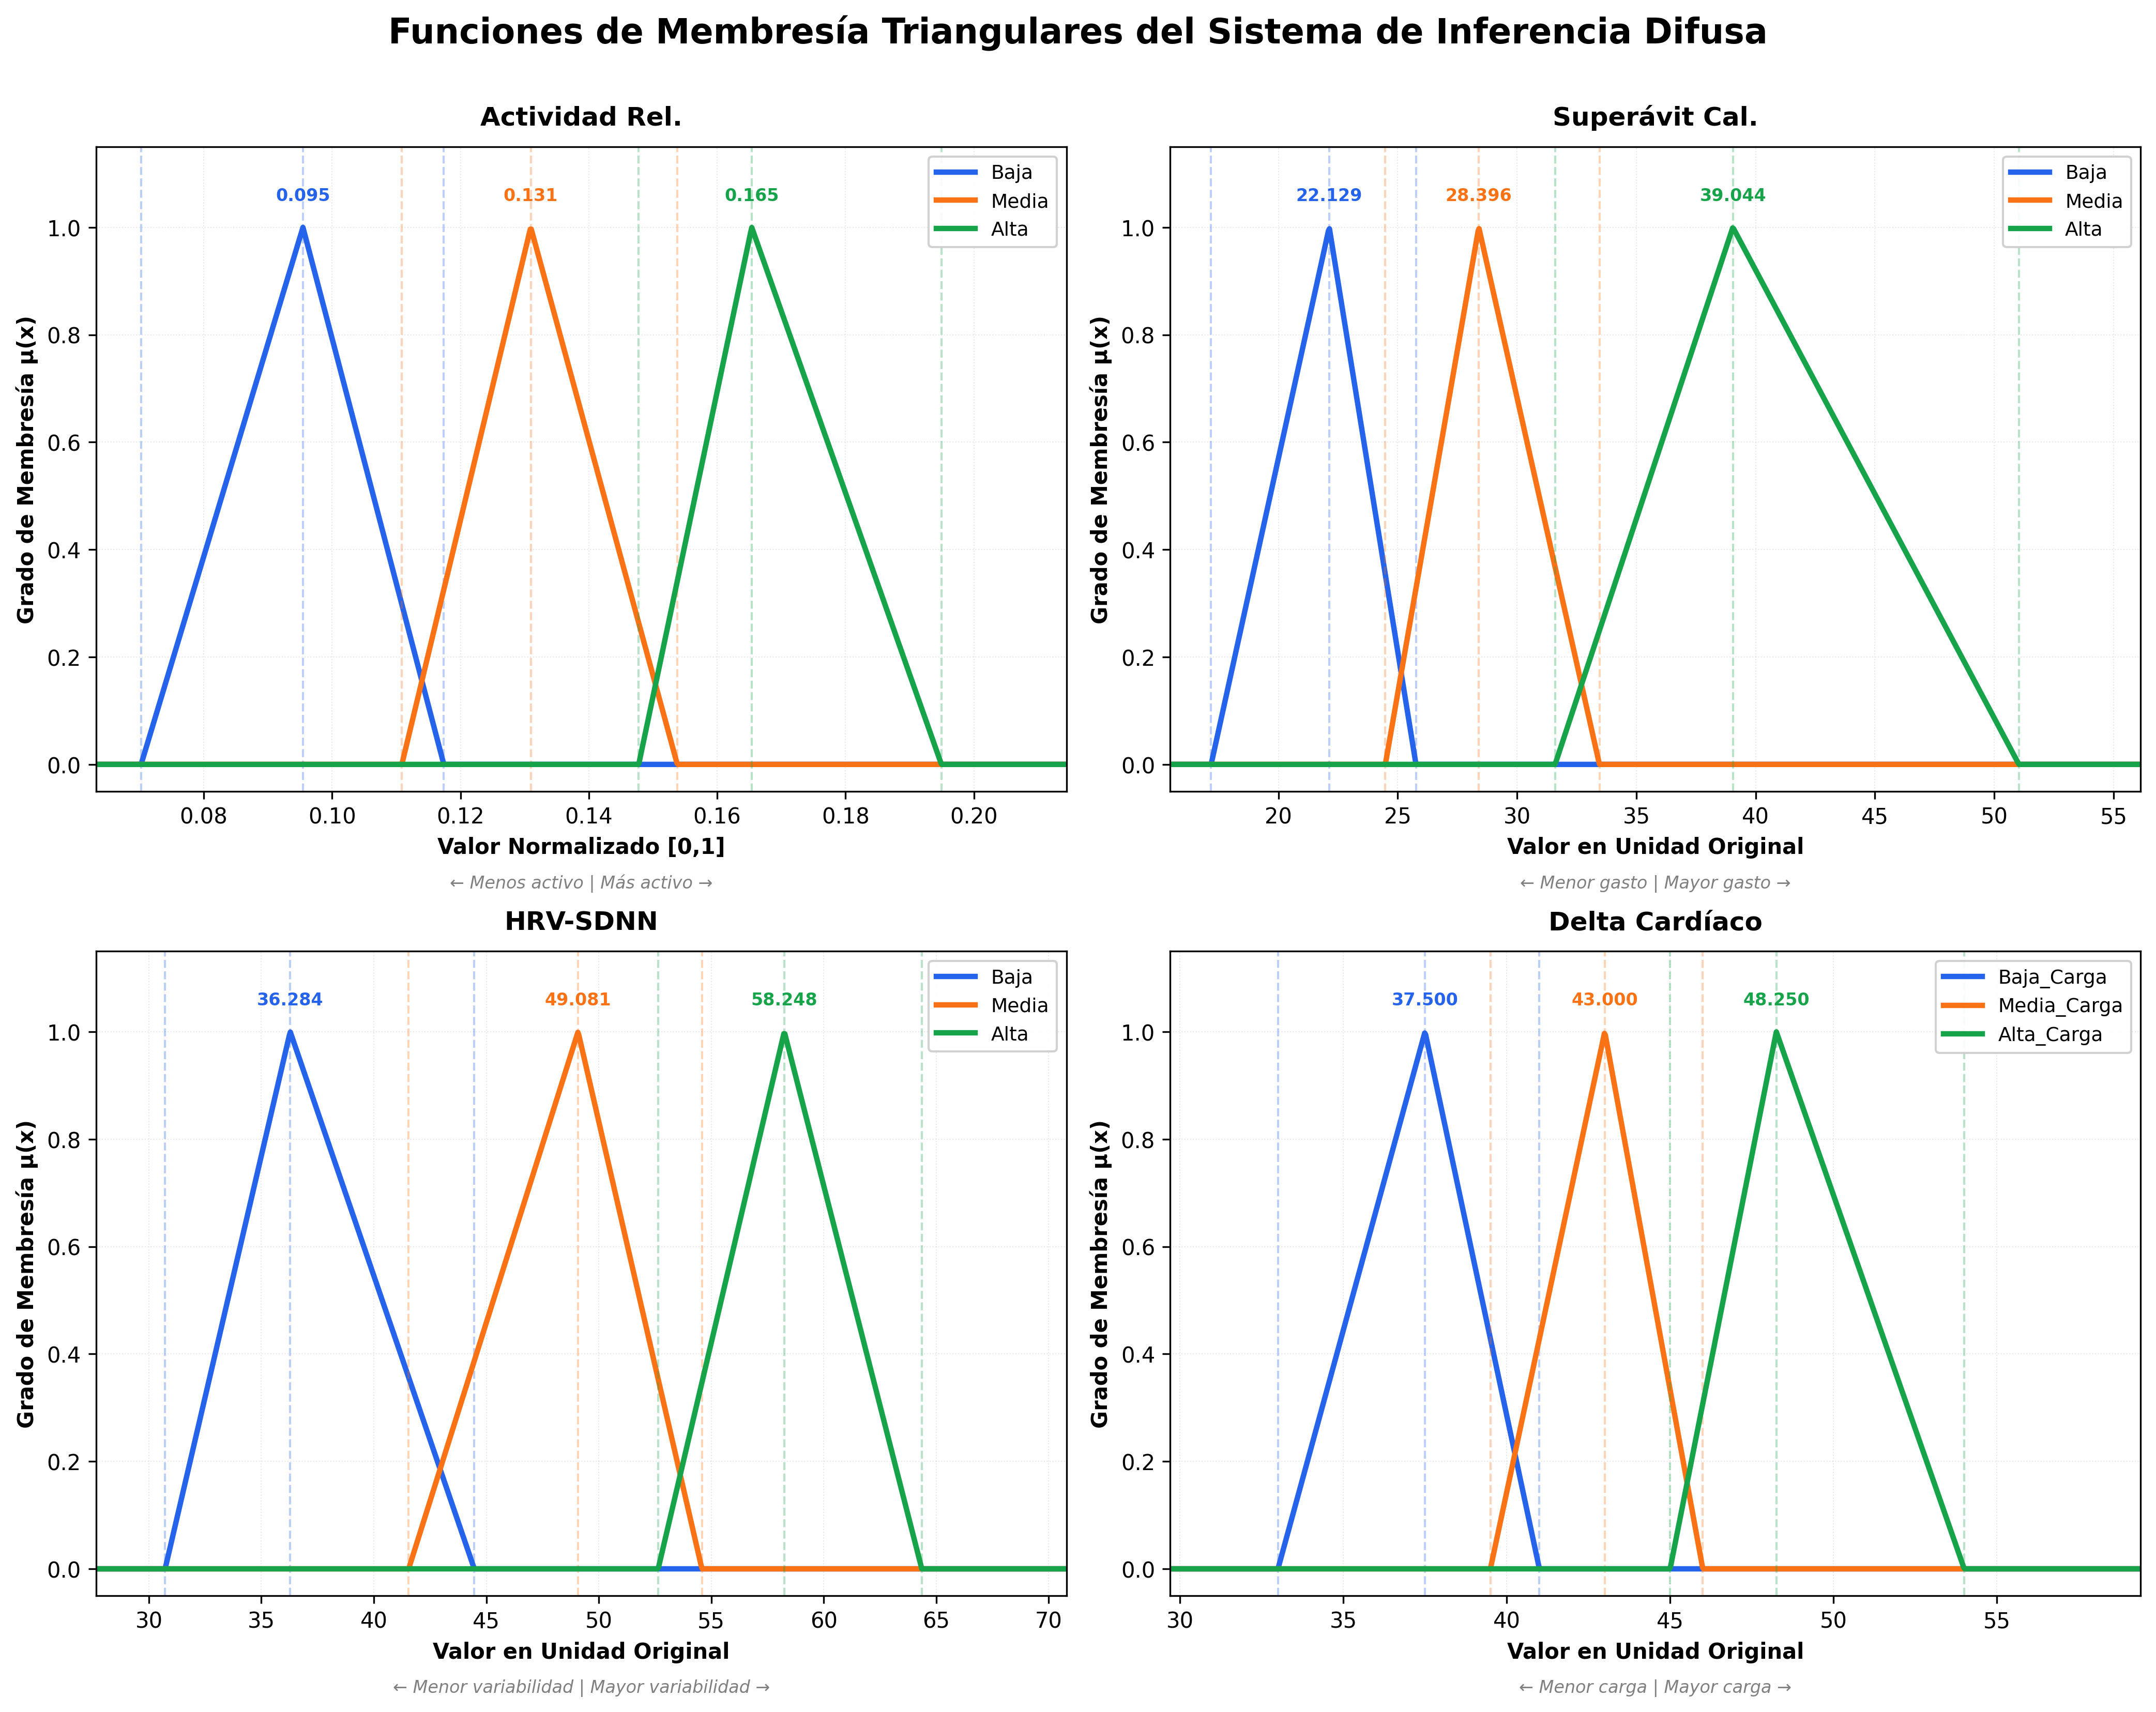
\includegraphics[width=0.95\textwidth]{figuras/funciones_membresia_triangulares.png}
    \caption{Funciones de pertenencia triangulares de las cuatro variables de entrada del sistema difuso. Los vértices (a, b, c) de cada triángulo fueron determinados mediante percentiles empíricos (P\textsubscript{10}, P\textsubscript{25}, P\textsubscript{40} para \textit{Baja}; P\textsubscript{35}, P\textsubscript{50}, P\textsubscript{65} para \textit{Media}; P\textsubscript{60}, P\textsubscript{75}, P\textsubscript{90} para \textit{Alta}), calculados sobre el conjunto de datos completo (N=10 usuarios, 1,337 semanas válidas). Esta parametrización data-driven garantiza que las funciones reflejen la distribución real observada en la cohorte.}
    \label{fig:funciones_membresia}
\end{figure}

Por ejemplo, podríamos definir un conjunto difuso ``actividad relativa baja'' donde $\mu_{\text{Baja}}(x) = 0.8$ para $x = 0.08$ (normalizado), significando que un valor de 0.08 se considera con un 80\% de pertenencia al concepto ``baja actividad''. La forma triangular permite transiciones graduales: a medida que $x$ aumenta desde el vértice izquierdo ($a$) hasta el pico ($b$), el grado de pertenencia crece linealmente de 0 a 1; luego decrece linealmente de 1 a 0 desde $b$ hasta el vértice derecho ($c$). Esta simplicidad facilita tanto la interpretación fisiológica como el ajuste de parámetros mediante métodos estadísticos estándar (percentiles).

Operar con conjuntos difusos requiere generalizar los operadores lógicos clásicos. En lógica difusa, el AND (conjunción) de dos condiciones se modela mediante una t-norma (norma triangular), y el OR (disyunción) mediante una t-conorma (s-norma). Estas operaciones combinan los grados de verdad de los operandos siguiendo ciertas propiedades (conmutatividad, asociatividad, monotonía y existencia de elementos neutro y nulo). La elección más común --por su simplicidad y significado intuitivo-- es usar la mínima (min) como t-norma para AND y la máxima (máx) como s-norma para OR. Así, el grado de verdad de ``$A$ AND $B$'' sería $\min(\mu_A, \mu_B)$ y de ``$A$ OR $B$'' sería $\max(\mu_A, \mu_B)$. De igual forma, la negación (NOT) de un conjunto difuso se define usualmente como el complemento estándar $\mu_{\neg A}(x) = 1 - \mu_A(x)$. Estas operaciones extienden las leyes de De Morgan al caso difuso, permitiendo cálculos lógicos coherentes con valores de verdad parciales.

Con estos elementos, es posible construir reglas difusas del tipo SI-ENTONCES para capturar conocimiento experto. Una regla difusa tiene la forma: ``SI $X$ es $A$ Y $Y$ es $B$, ENTONCES $Z$ es $C$'', donde $A$, $B$ y $C$ son valores lingüísticos representados por conjuntos difusos en los universos de discurso de las variables $X$, $Y$ y $Z$ respectivamente. Por ejemplo, una regla en nuestro contexto podría ser: ``SI actividad relativa es baja Y superávit calórico es bajo, ENTONCES sedentarismo es alto''. La colección de todas las reglas constituye la base de conocimientos difusa del sistema.

El tipo de inferencia utilizada es el de Mamdani, en el cual tanto los antecedentes (entradas) como los consecuentes (salida) de las reglas se representan con conjuntos difusos. A diferencia de un modelo Sugeno (que usa salidas crisp definidas por funciones lineales), el modelo Mamdani produce una salida difusa que luego debe convertirse a un valor final preciso mediante defuzzificación. La \Cref{fig:salida_difusa} ilustra este proceso: el motor de inferencia combina las reglas activadas y genera una distribución difusa de salida, la cual se defuzzifica mediante el método del promedio ponderado (weighted average) para obtener un valor numérico interpretable. Esta elección metodológica de defuzzificación (promedio ponderado en lugar del centroide clásico) se justifica por su menor complejidad computacional y mayor estabilidad numérica cuando múltiples reglas se activan simultáneamente con pesos similares.

\begin{figure}[htbp]
    \centering
    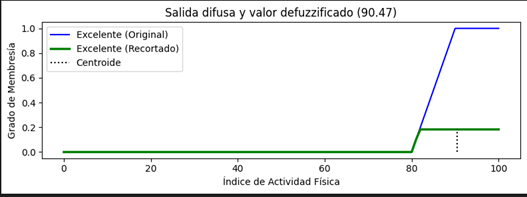
\includegraphics[width=0.85\textwidth]{figuras/Salida_difusa_figura_5.png}
    \caption{Proceso de defuzzificación del sistema de inferencia Mamdani}
    \label{fig:salida_difusa}
\end{figure}

En resumen, matemáticamente el sistema consta de: (a) conjuntos difusos y funciones de pertenencia \textbf{triangulares} que definen las etiquetas lingüísticas para cada variable mediante parametrización data-driven (percentiles empíricos); (b) operadores lógicos difusos (t-normas, s-normas, negadores) que permiten evaluar la veracidad parcial de premisas compuestas; (c) un conjunto de cinco reglas SI ENTONCES difusas basadas en conocimiento fisiológico del ejercicio que relacionan las entradas (comportamientos sedentarios/activos medidos por sensores wearables) con la salida (índice de sedentarismo); y (d) un mecanismo de inferencia difusa Mamdani que combina las reglas mediante t-norm de Gödel (mínimo) y obtiene una salida difusa, la cual finalmente se transforma en un valor numérico mediante defuzzificación por promedio ponderado.

% ============================================================================
% NOTA CRÍTICA: Esta sección introductoria ahora es coherente con:
% - fuzzy_membership_config.yaml (fuente operativa)
% - Formalización matemática rigurosa (subsección siguiente)
% - Figura actualizada con funciones triangulares
% ============================================================================


